\documentclass[hyperref={bookmarksopen=false}]{beamer} 

\usepackage[english]{babel}
\usepackage{pgf,pgfarrows,pgfnodes,pgfautomata,pgfheaps,pgfshade}
\usepackage[latin1]{inputenc}
\usepackage{graphicx}

\useoutertheme[section]{tubs}

%\setbeamertemplate{itemize items}[ball]
%\setbeamertemplate{itemize items}[square]
\setbeamertemplate{itemize items}[tusquare]

\title{Labor Android Programmierung - 1. Review}
\subtitle{LDAP Contact Sync} 
\author{Till Lorentzen und Christopher Gerloff}
\institute[TU Braunschweig, IBR]{Technische Universit�t Braunschweig, IBR}

\date{\today}

\instlogo{ibr_deu}
%\titlegraphic{iz}
\titlegraphic{iz_corner}



\begin{document}

\frame[plain]{\titlepage} 

\setbeamercolor{frametitle}{fg=white,bg=tu-red}
\frame{
        \frametitle{Einleitung}
        \tableofcontents
        }
\setbeamercolor{frametitle}{fg=black,bg=tu-grey}


\section{Einleitung}

\frame{
 \frametitle{Einleitung} 
 \begin{block}{Idee}
 \begin{itemize}
     \item Kontaktsynchronisation mit LDAP Verzeichnissen
 \end{itemize}
 \end{block}
 \begin{block}{Aufgaben}
    \begin{itemize}
        \item Gibt es funktionierende LDAP Bibliotheken fuer Java/Android?
        \item Wie soll die Anwendung strukturiert sein?
        \item Welche Funktionen soll die Anwendung bereitstellen?
        \item Wie Importieren/Exportieren/Synchronisieren wir die Kontaktdaten?
        \item Design der grafischen Oberflaeche
        \item Aufsetzen eines LDAP Servers zum Testen
    \end{itemize}
 \end{block}
}

\section{Stand der Dinge}

\frame{
	\frametitle{Stand der Dinge}
	
 	  \begin{block}{Bisherige Ergebnisse}
   	      \begin{itemize}
                  \item Zwei LDAP Bibliotheken fuer Java
                    \begin{itemize}
                      \item JOpenLDAP
                      \item LDAP SDK von UnboundID
                    \end{itemize}
                  \item Struktur der Anwendung ist festgelegt
                  \item Primaere Funktionen sind definiert
                  \item Importieren/Exportieren/Synchronisieren in Arbeit
                  \item Prototyp der grafischen Oberflaeche erstellt
                  \item LDAP Server noch nicht aufgsetzt
                   \begin{itemize}
                      \item Testen der Verbindung bisher mit oeffentlichen LDAP Verzeichnissen
                    \end{itemize}
                \end{itemize}
           \end{block}
}

\begin{frame}[fragile]
	\frametitle{Grafische Oberflaeche}
	\begin{block}{Hauptbildschirm}
	\hspace{0.5 cm}
	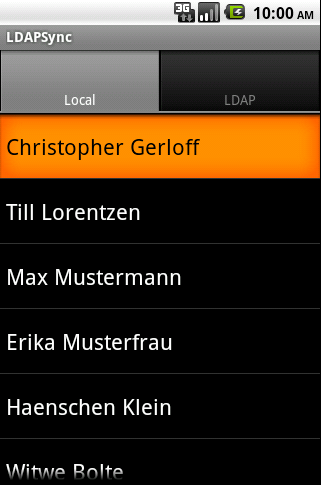
\includegraphics[scale=0.3]{LocalTabView.png}
	\vspace{1 cm}
	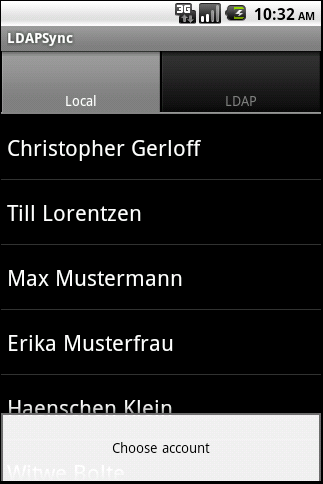
\includegraphics[scale=0.3]{LocalTabView_MenuOpen.png}
	\vspace{1 cm}
	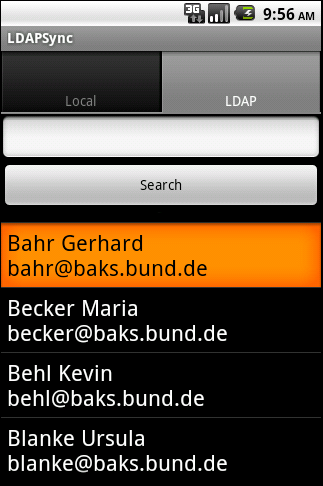
\includegraphics[scale=0.3]{LDAPTabView.png}
	\end{block}
\end{frame}

\begin{frame}[fragile]
	\frametitle{Grafische Oberflaeche}
	\begin{block}{Kontoverwaltung}
	\hspace{0.5 cm}
	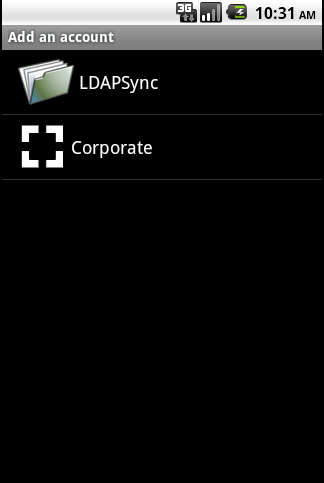
\includegraphics[scale=0.3]{Add_Account_AccountsandSync.png}
	\vspace{1 cm}
	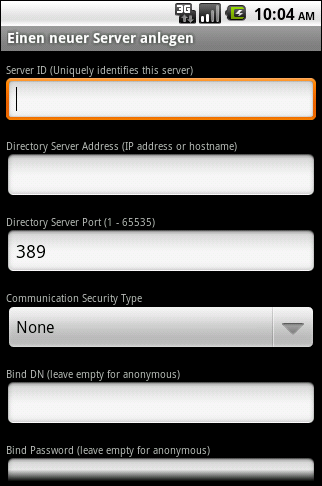
\includegraphics[scale=0.3]{Add_Account1.png}
	\vspace{1 cm}
	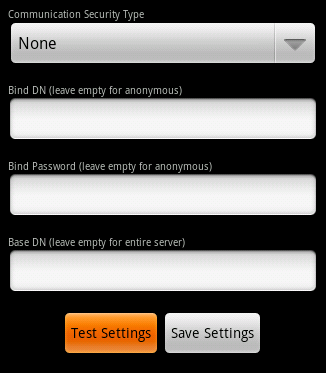
\includegraphics[scale=0.3]{Add_Account2.png}
	\end{block}
\end{frame}

\begin{frame}[fragile]
	\frametitle{Grafische Oberflaeche}
	\begin{block}{Integrierte Erweiterungen}
	\hspace{0.5 cm}
	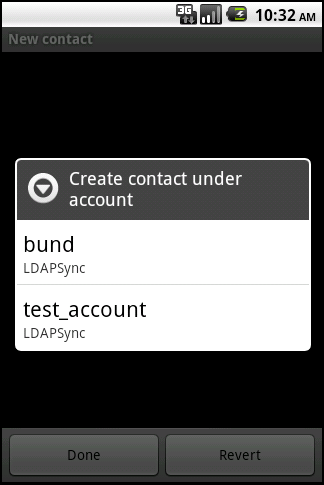
\includegraphics[scale=0.3]{createContact_chooseAccount.png}
	\vspace{1 cm}
	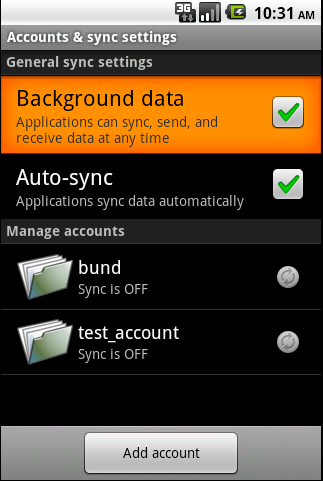
\includegraphics[scale=0.3]{Accounts_Sync.png}
	\end{block}
\end{frame}

\begin{frame}[fragile]
	\frametitle{Grafische Oberflaeche}
	\begin{block}{Sonstiges}
	\hspace{0.5 cm}
	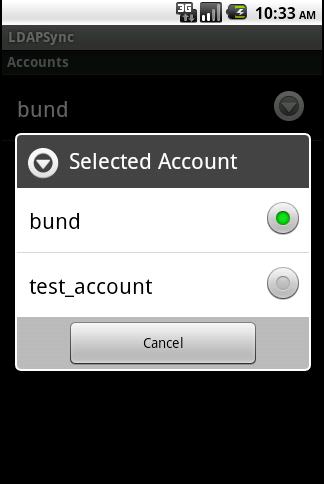
\includegraphics[scale=0.3]{choose_active_Account_for_TabView.png}
	\vspace{1 cm}
	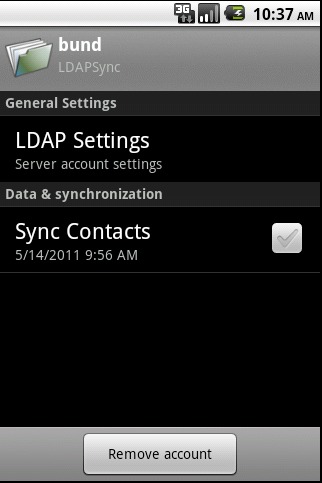
\includegraphics[scale=0.3]{specific_Account_Settings.png}
	\end{block}
\end{frame}

\frame{
 \frametitle{Wichtige Komponenten} 
 \begin{block}{AccountManager}
 \begin{itemize}
     \item Bla
 \end{itemize}
 \end{block}
 \begin{block}{SyncAdapter}
    \begin{itemize}
        \item Bla
    \end{itemize}
 \end{block}
  \begin{block}{RawContacts}
    \begin{itemize}
        \item Bla
    \end{itemize}
 \end{block}
}

\frame{
 \frametitle{Wichtige Komponenten} 
    \begin{block}{AccountAuthenticator}
    \begin{itemize}
        \item Bla
    \end{itemize}
 \end{block}
   \begin{block}{ContentProvider}
    \begin{itemize}
        \item Bla
    \end{itemize}
 \end{block}
}

\section{Ausblick}

\frame{
 \frametitle{Ausblick} 
 \begin{block}{To Do}
 \begin{itemize}
     \item Bla
 \end{itemize}
 \end{block}
}

\end{document}   
